\section{Role Based Access Control}

Diese Pattern basiert stark auf dem Authorization Pattern und versucht dessen Nachteile durch einen zusätzlichen Abstraktionslayer auszugleichen.
Das ''Role Based Access Control'' Pattern definiert Berechtigungen nicht direkt auf Stufe der Subjekte, sondern versucht diese in Gruppen (Aufgabenbereiche, Kaderposition, Arbeitsort etc.) einzuteilen und anschliessend auf dieser Ebene quasi übergeordnet zu berechtigen.

\subsection*{Kontext}
Eine Umgebung mit vielen Objekten und Subjekten. Deren Berechtigungen ändern häufig. Zudem ist damit zu rechnen dass eben so oft neue Subjekte und Objekte hinzukommen oder wieder wegfallen.

\subsection*{Problem}
Die Rechteverwaltung in dem beschriebenen Kontext generiert einen hohen administrativen Aufwand. Um die Anzahl individueller Berechtigungen zu minimieren soll versucht werden, alle Subjekte in Gruppen einzuteilen. Die Einteilung basiert darauf, dass Subjekte mit ähnlichen Aufgaben zumeist auch ähnliche oder identische Berechtigungen benötigen.
Trotzdem sollen die Berechtigungen weiterhin präzise abgebildet werden können (''Need to know'').

\subsection*{Lösung}
Organisationen bieten normalerweise bereits mehr oder weniger wohldefinierte Gruppenstrukturen (Abteilungen, Aufgabenbereiche).
Ein gutes Sicherheitskonzept sollte bestrebt sein, dass jedes Subjekt genau auf die Objekte Zugriff hat, mit welchen es täglich arbeitet (wiederum ''Need to know'').

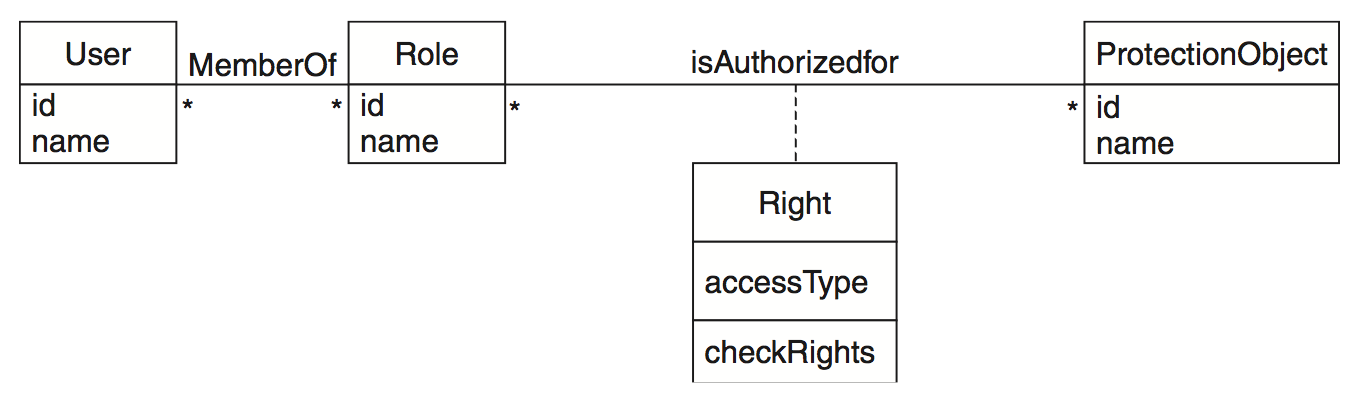
\includegraphics[width=\textwidth]{chapter/01basic/rolebasedaccesscontrol.png}

Im Vergleich zum Authorization Pattern kommt lediglich ein neues Element hinzu: Die Role fasst mehrere User (Subjekte) zu einer Menge zusammen und berechtigt sie über Right für ein spezifisches ProtectionObject.


\subsection*{Erweiterungen}
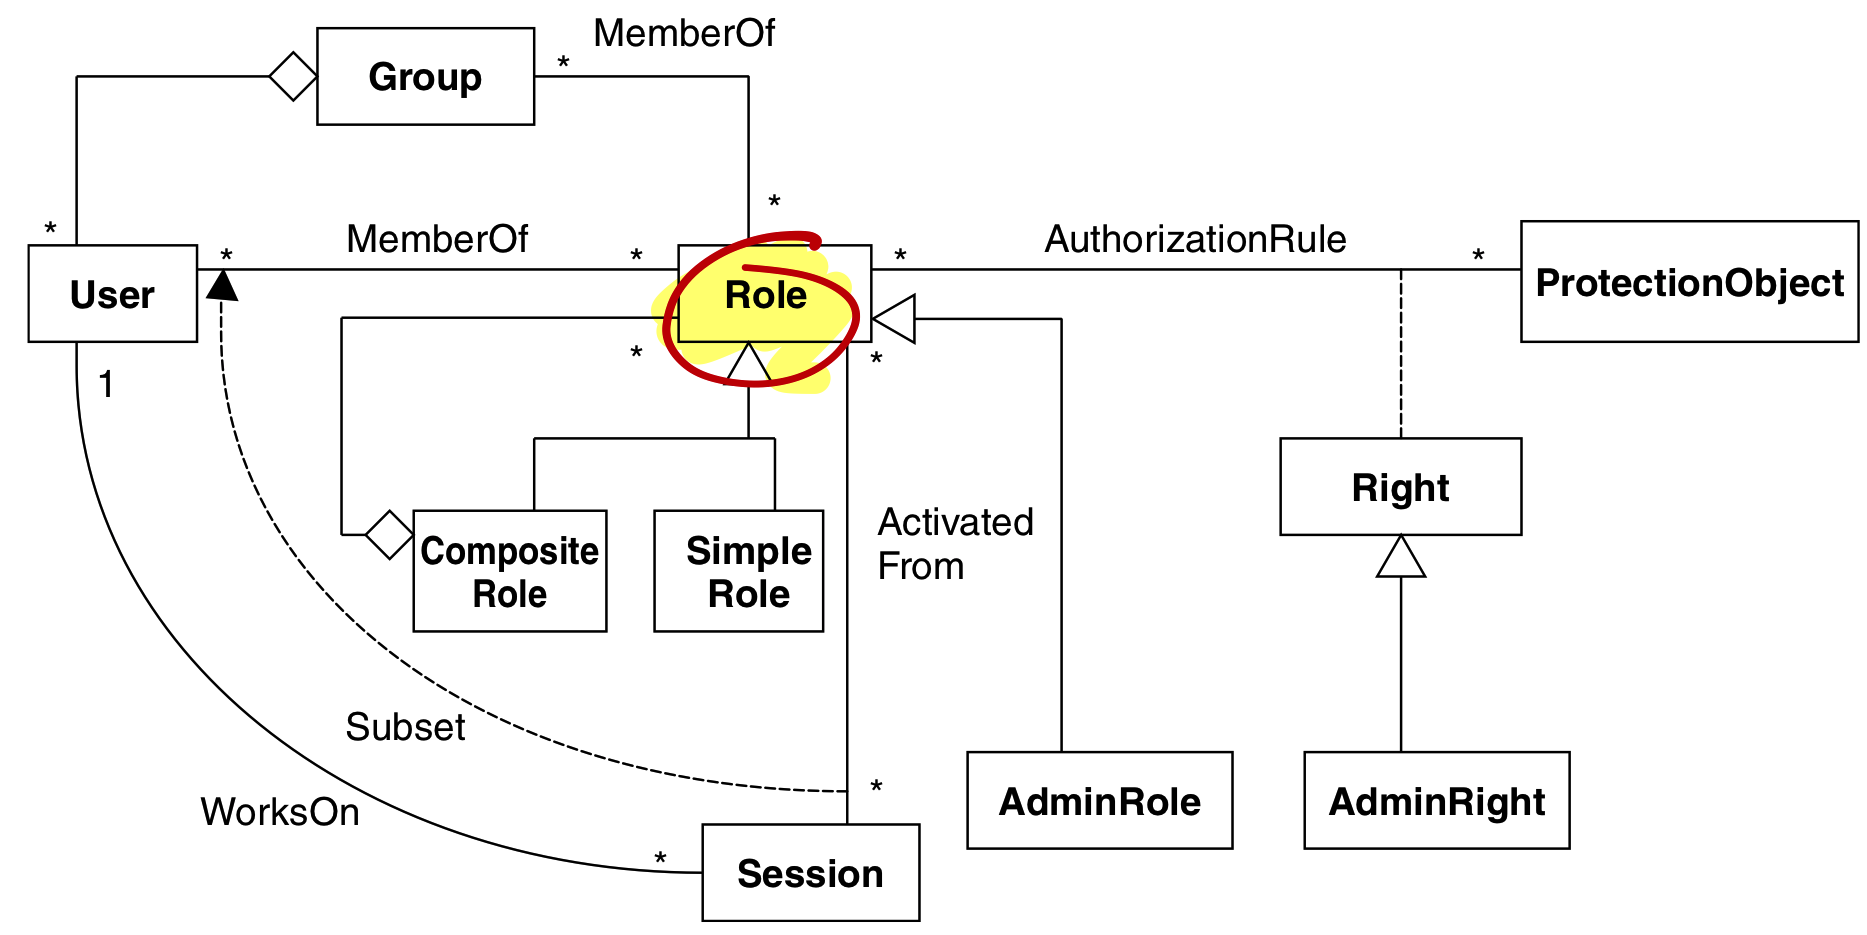
\includegraphics[width=\textwidth]{chapter/01basic/rolebasedaccesscontroladvanced.png}

\subsubsection*{Composite Pattern}
Statt einer simplen Assoziation zwischen User und Role könnte auch mit dem Composite-Pattern gearbeitet werden, um diese Abhängigkeit zu modellieren.

\subsubsection*{Administration}
Wie ebenfalls bereits im Authorization-Pattern erwähnt kann auch dieses Modell zielgerichtet um Administrations-Elemente erweitert werden.
Auf diese Weise kann zusätzliche Klarheit im System geschaffen werden, wer genau für was zuständig ist.

\subsubsection*{Abstract Session}
Um die Möglichkeiten auf die Spitze zu treiben, sei hier auch das Abstract Session Pattern erwähnt: Die Abhängigkeit einer Session kann so direkt ins Security Modell ''miteinmodelliert'' werden.

\subsection*{Vor- \& Nachteile}
\begin{itemize}
	\item 
\end{itemize}

\subsection*{Beispielanwendungen}
\begin{itemize}
	\item 
\end{itemize}